\documentclass[10pt]{article}
\usepackage[utf8]{inputenc}
\usepackage[T1]{fontenc}
\usepackage{amsmath}
\usepackage{amsfonts}
\usepackage{amssymb}
\usepackage[version=4]{mhchem}
\usepackage{stmaryrd}
\usepackage{hyperref}
\hypersetup{colorlinks=true, linkcolor=blue, filecolor=magenta, urlcolor=cyan,}
\urlstyle{same}
\usepackage{graphicx}
\usepackage[export]{adjustbox}
\graphicspath{ {./images/} }
\usepackage{caption}

\title{A flexible model for water based on TIP4P/2005 }

\author{Miguel A. González and José L. F. Abascal ${ }^{\text {a) }}$\\
Departamento de Química Física, Facultad de Ciencias Químicas, Universidad Complutense de Madrid, 28040 Madrid, Spain}
\date{}


%New command to display footnote whose markers will always be hidden
\let\svthefootnote\thefootnote
\newcommand\blfootnotetext[1]{%
  \let\thefootnote\relax\footnote{#1}%
  \addtocounter{footnote}{-1}%
  \let\thefootnote\svthefootnote%
}

%Overriding the \footnotetext command to hide the marker if its value is `0`
\let\svfootnotetext\footnotetext
\renewcommand\footnotetext[2][?]{%
  \if\relax#1\relax%
    \ifnum\value{footnote}=0\blfootnotetext{#2}\else\svfootnotetext{#2}\fi%
  \else%
    \if?#1\ifnum\value{footnote}=0\blfootnotetext{#2}\else\svfootnotetext{#2}\fi%
    \else\svfootnotetext[#1]{#2}\fi%
  \fi
}

\def\AA{\mathring{\mathrm{A}}}

\DeclareUnicodeCharacter{22EF}{\ifmmode\cdots\else{$\cdots$}\fi}

\begin{document}
\maketitle
\captionsetup{singlelinecheck=false}
(Received 29 July 2011; accepted 2 November 2011; published online 14 December 2011)

\begin{abstract}
A new flexible water model, TIP4P/2005f, is developed. The idea was to add intramolecular degrees of freedom to the successful rigid model TIP4P/2005 in order to try to improve the predictions for some properties, and to enable the calculation of new ones. The new model incorporates flexibility by means of a Morse potential for the bond stretching and a harmonic term for the angle bending. The parameters have been fitted to account for the peaks of the infrared spectrum of liquid water and to produce an averaged geometry close to that of TIP4P/2005. As for the intermolecular interactions, only a small change in the $\sigma$ parameter of the Lennard-Jones potential has been introduced. The overall predictions are very close to those of TIP4P/2005. This ensures that the new model may be used with the same confidence as its predecessor in studies where a flexible model is advisable.
\end{abstract}

© 2011 American Institute of Physics. [doi:10.1063/1.3663219]

\section*{I. INTRODUCTION}
Given the importance of water, it seems pertinent to understand the interaction between water molecules in the condensed phase. Several successful interaction potentials have been developed in the past. Simulation studies show that these force fields account for many important properties of liquid water although, needless to say, there is still room for improvement. ${ }^{1,2}$ A common feature of the most popular water models is that they are rigid, i.e., the intramolecular degrees of freedom are frozen. It may seem obvious that a step forward for the improvement of the water potential would be the addition of flexibility. However, there has been some skepticism on the past about the usefulness of flexible water models. ${ }^{3-6}$ In fact, Tironi et al. ${ }^{4}$ concluded that the introduction of flexibility creates more problems than it solves and does not improve upon the accuracy of rigid models. Notice that the high frequency of the bond stretching forces one to use a time step about five times smaller than that of a rigid model. In this way, the performance of flexible models may not justify its increased computational cost. It may be argued that flexible models make possible the calculation of new properties. But that must be done with care because the high frequency of the new accessible vibrational modes indicates that these are strongly quantized. In this context, a flexible model would be more justified in the case of a quantum treatment of the nuclear motion. In fact, interesting results have been obtained in quantum simulations of a flexible water model. ${ }^{7}$

However, rigid models do not allow to investigate certain properties, noticeably the infrared (IR) spectrum, that require the use of a flexible molecular geometry. This is important because computer simulations provide a set of instantaneous configurations of the system from which it is

\footnotetext{${ }^{\text {a) }}$ Author to whom correspondence should be addressed. Electronic mail: \href{mailto:bascal@quim.ucm.es}{bascal@quim.ucm.es}.
}
possible to get useful structural information that cannot be directly extracted from experiment. For instance, it enables the assignment of some bands of unclear origin appearing in the Raman spectrum of liquid water. Moreover, it enables a detailed analysis of the relationship between power spectrum and the hydrogen bonding network. ${ }^{8,9}$ A flexible model is also imperative in other situations as, for example, in the empirical valence bond methodology and its multistate generalization. ${ }^{10}$ Besides, there are a number of reports claiming that some predictions of flexible models are closer to experimental data than those of rigid potentials. ${ }^{11-15}$ Yuet and Blankschtein ${ }^{15}$ have concluded that the surface tension of water is determined by the delicate balance between intramolecular (bond stretching) and intermolecular (LJ) interactions. Raabe and Sadus ${ }^{12}$ have shown that introducing bond flexibility significantly improves the prediction of both the dielectric constants and the equation of state of liquid water. These authors argue that adding intramolecular degrees of freedom to a rigid water model introduces in some way the effect of the local environment. This is because the changes in the molecular geometry in response to the thermodynamic state point produce variations in the dipole moment. Thus, the fluctuations in the total dipole moment of the system come not only from the variations in the relative orientation of the molecules (as in a rigid model) but also from the changes in the dipole moment of the molecules. In this way, the variation of the dielectric constant as a consequence of changes in the environment of the molecules could be better described with a flexible model than with a rigid one (notice also that the ability of a flexible model to vary in a changing environment could be, in principle, of great value in the study of interfaces.) On the other hand, flexible bonds and angles are required when dealing with systems with torsional degrees of freedom. Consequently, the forcefields employed in biomolecular simulations contain terms according with this need. Although many authors prefer to use a rigid water model in these conditions, some of them find more consistent to use also a flexible water model. In summary, despite the skepticism of several reports, there are some reasons\\
supporting the interest in developing (or improving) flexible water models.

It seems natural that the development of flexible models will consist on the addition of flexibility to a successful rigid potential. Until recently, it has been a general feeling that two models, namely, TIP4P (Ref. 16) and SPC/E, ${ }^{17}$ provided the best ratio between performance and simplicity. However, recent investigations on the phase diagram involving the solid phases of water have demonstrated ${ }^{18-21}$ the superiority of the charge distribution of TIP4P model over that of SPC/E. For this reason, an updated version of TIP4P including intramolecular degrees of freedom could of interest for those investigating water properties that require the use of a flexible model. On the other hand, the idea behind the parametrization of SPC/E (a correction term is added to the enthalpy of vaporization) seems to be responsible for the good predictions of this model. In this way, TIP4P and SPC/E obtain similar scores in a recently reported performance analysis of water models. ${ }^{2}$ It was evident that the water force field could be improved by merging the relevant features of both models. This is in essence the basis of the success of TIP4P/2005. ${ }^{22}$ Since its proposal, a rather comprehensive set of properties has been evaluated for this model. It provides an excellent agreement with experiment for thermodynamic, ${ }^{22-24}$ structural, ${ }^{25,26}$ and dynamical ${ }^{27,28}$ properties, over a wide range of temperatures from subcritical ${ }^{29}$ to the liquid-gas critical point. Its performance has also been contrasted with experiment in the case of biomolecular systems. ${ }^{30}$ Because of this, the goal of this work is to develop a flexible version of TIP4P/2005.

This article is organized as follows: In Sec. II we give the details of our choice for the intramolecular interactions and present the parameters of the new model (which we term as TIP4P/2005f) as well as the averaged geometry in the liquid state. In Sec. III we discuss the results obtained in molecular dynamics simulations of the model which are compared with experiment and with those for TIP4P/2005. Finally, conclusions are given in Sec. IV.

\section*{II. THE MODEL}
A number of computer simulations with different flexible water models have been reported ${ }^{8,11,31-34}$ since the pioneering works of Lemberg and Stillinger ${ }^{35}$ and Toukan and Rahman. ${ }^{36}$ As commented in the introduction it seems convenient to develop a new flexible model based on the rigid water model TIP4P/2005. The first problem we face is the choice of the character of this flexibility, namely, harmonic or anharmonic. The use of a harmonic function $V_{\mathrm{OH}_{i}}=D_{r} \beta^{2}\left(r_{\mathrm{OH}_{i}}-r_{\mathrm{eq}}\right)^{2}$ may be advised because it is computationally less expensive. Figure 1 compares the harmonic potential for the bond stretching with the cubic and quartic ones as well as the full Morse potential. All functions have the minimum at the same distance but the interaction differs significantly as one moves away from equilibrium. When calculating the power spectrum with the harmonic potential we observed a splitting in the OH stretching band ( $\sim 3400 \mathrm{~cm}^{-1}$ ) which did not correspond with the experimental data. ${ }^{37,38}$ In the case of using anharmonic functions, the splitting of the band disappeared and was closer to experiment. For this reason we chose an anharmonic func-

\begin{figure}[h]
\begin{center}
  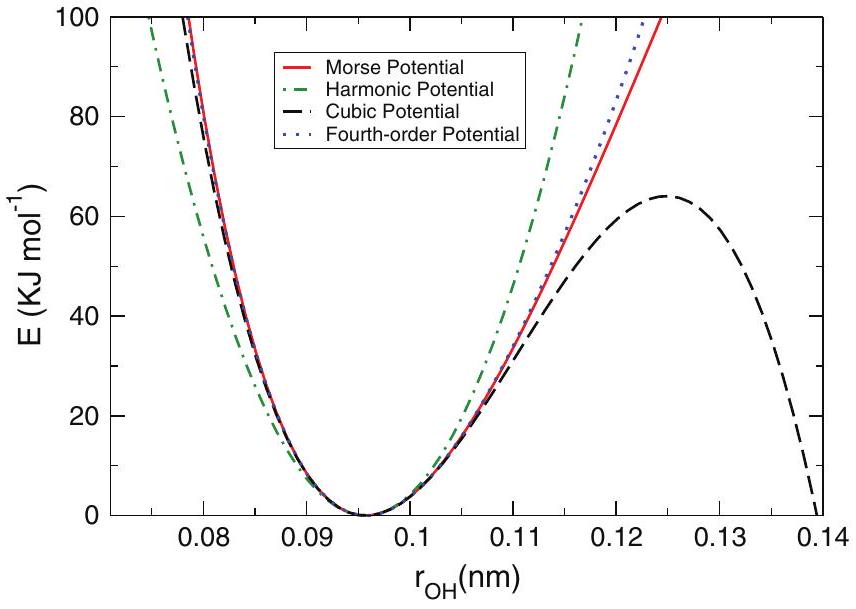
\includegraphics[alt={},max width=\textwidth]{a79b7aee-e943-46ce-b653-92f3182dbe04-3_609_856_176_1091}
\captionsetup{labelformat=empty}
\caption{FIG. 1. Four alternative functions to describe the bond stretching in a flexible water model.}
\end{center}
\end{figure}

tion to represent the flexibility of the OH bond. Once the harmonic potential is ruled out, it can be seen in Fig. 1 that the cubic function exhibits a wiggle which can be problematic in computer simulation. The quartic and Morse functions are quite similar even at distances relatively far from equilibrium. We finally opted for the full Morse function because the calculations indicated that its use did not increase the computational cost. The intramolecular potential is then given by


\begin{equation*}
V^{\text {intra }}=V_{\mathrm{OH}_{1}}(r)+V_{\mathrm{OH}_{2}}(r)+V_{\mathrm{HOH}}(\theta), \tag{1}
\end{equation*}



\begin{equation*}
V_{\mathrm{OH}_{i}}=D_{r}\left\{1-\exp \left[-\beta\left(r_{\mathrm{OH}_{i}}-r_{\mathrm{eq}}\right)\right]\right\}^{2}, \tag{2}
\end{equation*}


where $r_{\mathrm{eq}}$ and $\theta_{\mathrm{eq}}$ are the values of the bond length and angle at equilibrium and $r_{\mathrm{OH}_{i}}$ is the instantaneous distance between the hydrogen atom $i$ and the oxygen atom. $D_{r}$ and $\beta$ are the parameters of the Morse potential that determine the bond strength and width. For the angle bending, a harmonic function (with an associated strength constant $K_{\theta}$ ) seems to be sufficient


\begin{equation*}
V_{\mathrm{HOH}}(\theta)=\frac{1}{2} K_{\theta}\left(\theta-\theta_{\mathrm{eq}}\right)^{2} . \tag{3}
\end{equation*}


The molecular geometry of our model is given by a slight modification of the TIP4P/2005 parameters. This amendment is the result of incorporating the flexibility which produces a elongation of the OH distance and a reduction of the HOH angle. For this reason we chose a smaller bond distance at equilibrium ( $r_{\text {eq }}=0.9419 \AA$ ) and a larger angle ( $\theta_{\text {eq }}=107.4^{\circ}$ ) than those of TIP4P/2005 (Table I).

As for the intermolecular potential, we follow the usual choice of TIP4P-like models: a Lennard-Jones center at the position of the oxygen atom plus the electrostatic interaction given by two positive charges located at the hydrogen atoms and a compensating negative charge placed at the so-called M-site. Since the molecule is not rigid, the location of the M site is defined in terms of the positions of the hydrogen atoms:


\begin{equation*}
d_{\mathrm{OM}}=d_{\mathrm{OM}}^{\mathrm{rel}}\left(z_{\mathrm{OH}_{1}}+z_{\mathrm{OH}_{2}}\right) \tag{4}
\end{equation*}


where $z_{\mathrm{OH}_{1}}$ and $z_{\mathrm{OH}_{2}}$ are the distances to the oxygen of the hydrogen's projections along the HOH bisector, $z_{\mathrm{OH}_{\mathrm{i}}}$

\begin{table}[h]
\begin{center}
\captionsetup{labelformat=empty}
\caption{TABLE I. Potential parameters of the TIP4P/2005f and TIP4P/2005 water models. Notice that $r_{\text {eq }}$ and $\theta_{\text {eq }}$ define the rigid geometry of TIP4P/2005.}
\begin{tabular}{|l|l|l|}
\hline
Parameter & TIP4P/2005f & TIP4P/2005 \\
\hline
$\epsilon / k(\mathrm{~K})$ & 93.2 & 93.2 \\
\hline
$\sigma(\AA)$ & 3.1644 & 3.1589 \\
\hline
$q_{H}(\mathrm{e})$ & 0.5564 & 0.5564 \\
\hline
$d_{\text {OM }}^{\text {rel }}$ & 0.13194 & 0.13194 \\
\hline
$D_{r}(\mathrm{~kJ} / \mathrm{mol})$ & 432.581 & ⋯ \\
\hline
$r_{\text {eq }}(\AA)$ & 0.9419 & 0.9572 \\
\hline
$\beta\left(\mathrm{nm}^{-1}\right)$ & 22.87 & ⋯ \\
\hline
$\theta_{\text {eq }}(\mathrm{deg})$ & 107.4 & 104.52 \\
\hline
$K_{\theta}\left(\mathrm{kJ} /\left(\mathrm{mol} \mathrm{rad}^{2}\right)\right)$ & 367.810 & ⋯ \\
\hline
\end{tabular}
\end{center}
\end{table}

$=d_{\mathrm{OH}_{i}} \cos (\theta / 2)$. We have chosen the value for $d_{\mathrm{OM}}^{\text {rel }}$ so as to reproduce the distance $d_{\mathrm{OM}}$ in the TIP4P/2005 geometry (i.e., $d_{\mathrm{OH}}=0.9572, \theta=104.52$ and, thus, $d_{\mathrm{OM}}=0.1546$ ). As a result of the addition of flexibility and the changes in the average molecular geometry it produces, the intermolecular parameters may not be optimized ${ }^{39}$ and require a further tuning. We observed that the properties more related to the interaction energy did not change significantly while those dependent on the molecular size (the orthobaric densities in particular) were slightly shifted with respect to those of the rigid model. Thus, it has been necessary to increase the parameter $\sigma$ of the Lennard-Jones interaction while the rest of parameters are not altered from TIP4P/2005. The parameters of the TIP4P/2005f model are collected in Table I where we have also included for comparison the corresponding values for TIP4P/2005.

Figure 2 shows the normalized histogram of the distribution of bond distances for a single molecule at a temperature close to 0 K (the actual value is 2 K ) compared to that for bulk conditions. We have used here a small time-step, 0.1 fs , and the simulations lasted 10 ps . As can be expected for a classical solution of the equation for the intramolecular motion, the bond distribution for a single molecule has two maxima coincident with the turning points of the bond

\begin{figure}[h]
\begin{center}
  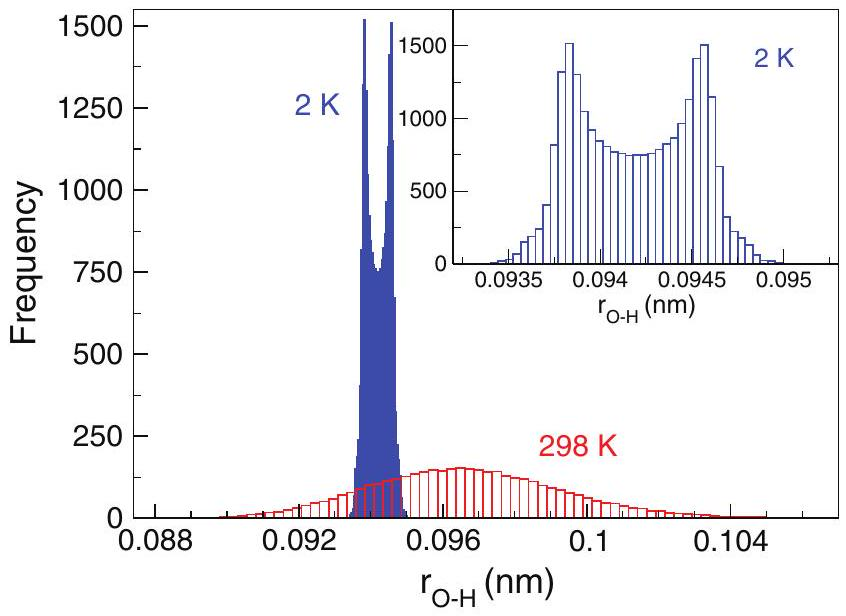
\includegraphics[alt={},max width=\textwidth]{a79b7aee-e943-46ce-b653-92f3182dbe04-4_616_846_1834_184}
\captionsetup{labelformat=empty}
\caption{FIG. 2. Distribution of bond distances at different conditions. The area of both histograms is normalized. The red (broader) histogram corresponds to liquid water at 1 bar, 298 K while the blue one corresponds to the results for a single molecule at 2 K (zoomed at the inset).}
\end{center}
\end{figure}

\begin{table}[h]
\begin{center}
\captionsetup{labelformat=empty}
\caption{TABLE II. Average value of the parameters related to the molecular geometry in a simulation at $T=298 \mathrm{~K}$ and $p=1 \mathrm{bar}$. The corresponding values for TIP4P/2005 are also given for comparison.}
\begin{tabular}{|l|l|l|}
\hline
Model & TIP4P/2005f & TIP4P/2005 \\
\hline
$\left\langle r_{\mathrm{OH}}\right\rangle(\AA)$ & 0.9664 & 0.9572 \\
\hline
$\left\langle r_{\mathrm{OM}}\right\rangle$ (Å) & 0.15555 & 0.1546 \\
\hline
$\langle\theta\rangle$ (deg) & 104.79 & 104.52 \\
\hline
$\langle\mu\rangle$ (D) & 2.319 & 2.305 \\
\hline
\end{tabular}
\end{center}
\end{table}

stretching (at this temperature the behavior corresponds approximately to a harmonic spring). This result is completely different from that given by quantum mechanics so one could question the validity of the results for the condensed state. But the collective effect of the intermolecular interactions dramatically change the distribution, which shows a more or less Gaussian profile in the liquid, in close agreement with quantum mechanical results. It is noticed that the maximum appears at distances larger than $r_{\text {eq }}$. For liquid water, the position of the peak depends slightly on the thermodynamic state. At room temperature and pressure, the value $r_{\text {eq }}=0.9419 \AA$ results in a maximum at $0.966 \AA$ (close to the fixed OH distance in TIP4P/2005).

Table II presents the average value along a simulation at ambient conditions of the parameters related to the molecular geometry, namely, bond distance $\left\langle r_{\mathrm{OH}}\right\rangle$, distance $\mathrm{O}-\mathrm{M}\left\langle r_{\mathrm{OM}}\right\rangle$, angle $\mathrm{H}-\mathrm{O}-\mathrm{H}\langle\theta\rangle$, and dipole moment $\langle\mu\rangle$. Also given are the corresponding values for the rigid model TIP4P/2005. It may be seen that the averaged molecular geometry of the model somewhat differs from that of the isolated molecule (cf. Table I and Fig. 2) but it is very close to that of TIP4P/2005.

\section*{III. RESULTS}
The simulations were carried out with the gromacs 4.0 package ${ }^{40,41}$ for a sample of 500 water molecules. When necessary we used the velocity-rescale thermostat, ${ }^{42}$ and the barostat of Parrinello-Rahman. ${ }^{43}$ The Lennard-Jones interactions were truncated at $8.0 \AA$. The particle mesh Ewald method ${ }^{44}$ was employed to calculate the long-range electrostatics forces. For the calculation of most of the properties discussed in this article we used a time step of 0.2 fs lasting 10 ns of total simulation time. In the event that we have used other conditions for the simulation we will describe it at the corresponding place in this article.

Table III presents a summary of the properties of the TIP4P/2005f water model at $T=298 \mathrm{~K}, p=1$ bar compared with experimental data and with the results for TIP4P/2005. We also present the melting point and the enthalpy of vaporization of the TIP4P/2005f model at room pressure. In the following we describe in more detail the properties of this new flexible model.

\section*{A. Liquid densities at normal pressure}
We have evaluated the density for the room pressure isobar at 12 different temperatures, from 250 K to 370 K . Numerical data are provided in Table IV and a plot of the

\begin{table}[h]
\begin{center}
\captionsetup{labelformat=empty}
\caption{TABLE III. A summary of the properties of TIP4P/2005f compared to the corresponding values for TIP4P/2005 and with experimental data. Density, $\rho$, isothermal compressibility, $\kappa_{T}$, (relative) static dielectric constant, $\varepsilon_{r}=\varepsilon / \varepsilon_{0}$, and self-diffusion coefficient, $D_{s}$, have been calculated at $T=298 \mathrm{~K}, p =1$ bar. The melting temperature, $\mathrm{T}_{m}$, and the enthalpy of vaporization, $\Delta_{v} H$, also correspond to a pressure of 1 bar. $\Delta_{v} H$ includes the self-polarization correction -Eq. (6)- while the values in parenthesis are the result of Eq. (5) without any further correction.}
\begin{tabular}{|l|l|l|l|}
\hline
Model & TIP4P/2005f & TIP4P/2005 & Expt. \\
\hline
$\rho\left(\mathrm{g} / \mathrm{cm}^{3}\right)$ & 0.9977 & 0.9979 & 0.9970 \\
\hline
$10^{5} \kappa_{T}\left(\mathrm{MPa}^{-1}\right)$ & 4.46 & 4.63 & 4.53 \\
\hline
$\varepsilon_{r}$ & 55.3 & 57.3 & 78.4 \\
\hline
$10^{9} D_{s}\left(\mathrm{~m}^{2} \mathrm{~s}^{-1}\right)$ & 1.93 & 2.08 & 2.27 \\
\hline
Melting temperature (K) & 254 & 252.1 & 273.15 \\
\hline
$\Delta_{v} H\left(\mathrm{KJ} \mathrm{mol}^{-1}\right)$ & 45.7(50.3) & 45.6 (50.1) & 44.05 \\
\hline
\end{tabular}
\end{center}
\end{table}

results is shown in Figure 3 where the characteristic "anomalous" behavior of water is clearly seen. The calculated densities are in excellent agreement with the experimental data. In fact, TIP4P/2005f performs even better than TIP4P/2005 for this property. Densities for the flexible model have been adjusted to a fifth-order polynomial. The temperature of maximum density (TMD) obtained with the fit is 280.3 K , only three degrees above the experimental value. As stated in several studies, ${ }^{2,45}$ an accurate prediction of the densities at room pressure and the TMD usually indicates that the model has an excellent performance in reproducing a wide variety of properties of liquid water.

\section*{B. Structure: Radial distribution function}
Oxygen-oxygen radial distribution function $g_{\mathrm{oo}}(r)$ is shown in Fig 4. TIP4P/2005f results are in general very close to the experimental data. ${ }^{46}$ Similarly to TIP4P/2005, it overestimates the height of the main peak and follows closely the experiment at larger distances. Minor differences between the results of both water models are seen at the first minimum where the flexible model results are slightly lower than those for TIP4P/2005 and at the second maximum where TIP4P/2005f performs slightly better.

\begin{table}[h]
\begin{center}
\captionsetup{labelformat=empty}
\caption{TABLE IV. Liquid densities (g/ $\mathrm{cm}^{3}$ ) at $p=1$ bar.}
\begin{tabular}{|l|l|l|}
\hline
T (K) & TIP4P/2005f & Expt. \\
\hline
250 & 0.9906 & 0.9913 \\
\hline
260 & 0.9959 & 0.9970 \\
\hline
270 & 0.9984 & 0.9995 \\
\hline
280 & 0.9997 & 0.9999 \\
\hline
290 & 0.9993 & 0.9988 \\
\hline
300 & 0.9971 & 0.9965 \\
\hline
315 & 0.9927 & 0.9915 \\
\hline
330 & 0.9862 & 0.9848 \\
\hline
340 & 0.9808 & 0.9795 \\
\hline
350 & 0.9748 & 0.9737 \\
\hline
360 & 0.9684 & 0.9674 \\
\hline
370 & 0.9615 & 0.9606 \\
\hline
\end{tabular}
\end{center}
\end{table}

\begin{figure}[h]
\begin{center}
  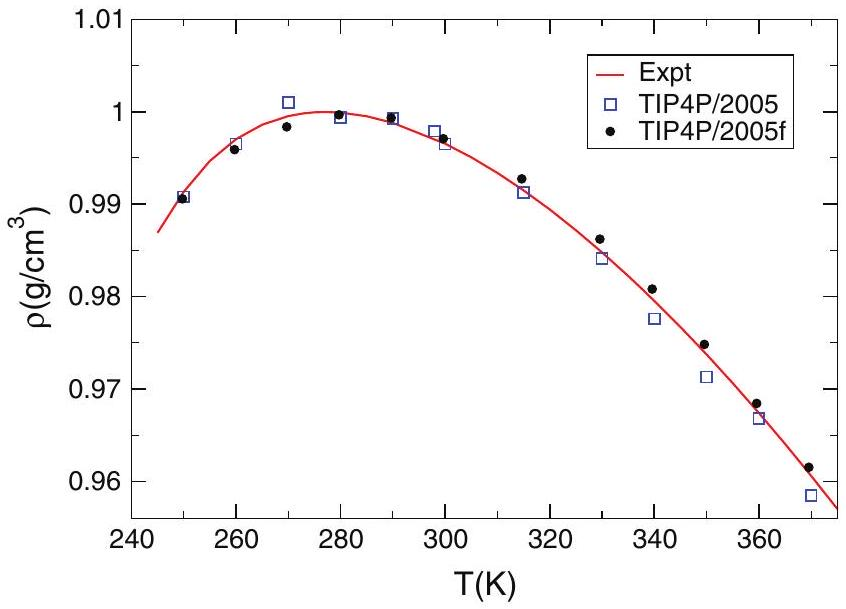
\includegraphics[alt={},max width=\textwidth]{a79b7aee-e943-46ce-b653-92f3182dbe04-5_609_846_171_1095}
\captionsetup{labelformat=empty}
\caption{FIG. 3. Densities of the TIP4P/2005f model (full circles) at $p=1$ bar compared to the values of the same property of TIP4P/2005 model (open squares) and experimental data (full line).}
\end{center}
\end{figure}

\section*{C. Enthalpy of vaporization}
The difference between the gas phase enthalpy minus the enthalpy of the liquid phase is known as enthalpy of vaporization, $\Delta_{v} H=H_{g}-H_{l}$. At low pressures the gas may be considered ideal and gives a negligible contribution to the internal energy. Besides, its volume may be calculated from the perfect gases equation. In this way, the enthalpy of vaporization may be approximated by


\begin{equation*}
\Delta_{v} H=-U_{l}-p V_{l}+R T . \tag{5}
\end{equation*}


The computed value for our model (Table III) is, by design, larger than the experimental result. This is because it is now widely accepted ${ }^{2}$ the need of the so-called self-energy correction proposed by Berendsen et al. ${ }^{17}$ This term should be subtracted from the enthalpy of vaporization to take into account the difference in polarization between the gas and the liquid phase. The correction depends on the difference between the dipole moment of the model $\mu_{l}$ and that of the gas phase $\mu_{g}$

\begin{figure}[h]
\begin{center}
  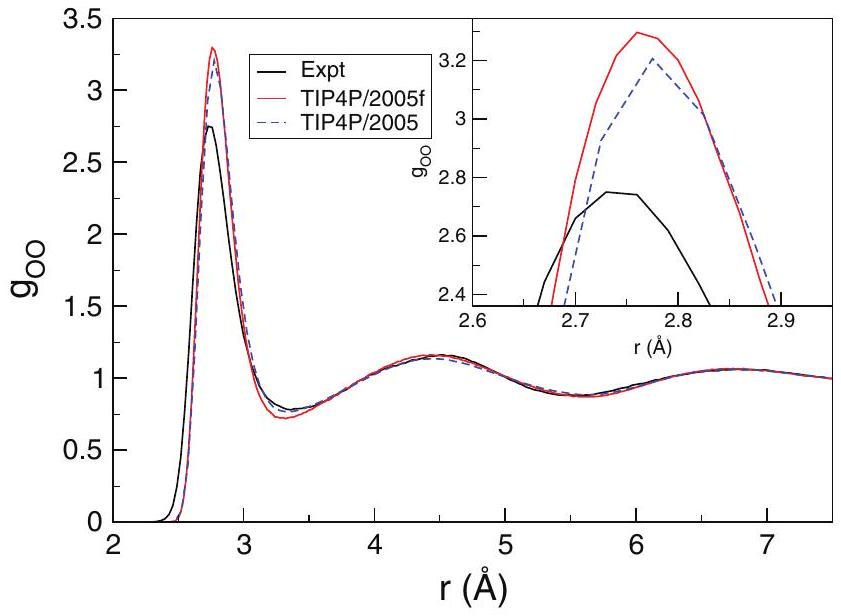
\includegraphics[alt={},max width=\textwidth]{a79b7aee-e943-46ce-b653-92f3182dbe04-5_616_841_1937_1100}
\captionsetup{labelformat=empty}
\caption{FIG. 4. Oxygen-oxygen radial distribution function at $T=298 \mathrm{~K}, p=1$ bar.}
\end{center}
\end{figure}

and may be approximated by


\begin{equation*}
\Delta E_{\mathrm{pol}}=\frac{\left(\mu_{l}-\mu_{g}\right)^{2}}{2 \alpha} . \tag{6}
\end{equation*}


Using the average dipole moment of the liquid at room temperature and temperature, the correction amounts to $4.6 \mathrm{~kJ} / \mathrm{mol}$. In these conditions, the enthalpy of vaporization is close to the experimental value.

\section*{D. Isothermal compressibility}
To calculate the isothermal compressibility we make use of the fluctuations equation


\begin{equation*}
\kappa_{T}=\frac{\left\langle V^{2}\right\rangle-\langle V\rangle^{2}}{k_{B} T\langle V\rangle}, \tag{7}
\end{equation*}


where $\langle V\rangle$ is the average volume, $k_{B}$ is the Boltzmann's constant and $T$ is the temperature. The value of $\kappa_{T}$ for our model is $(4.46 \pm 0.003) \times 10^{5} \mathrm{MPa}$ at 298 K and atmospheric pressure. This result is again similar to that for the TIP4P/2005 model but it is slightly closer to the experiment as it may be seen in Table III.

\section*{E. Self-diffusion coefficient}
The self-diffusion coefficient was calculated by means of the Einstein equation


\begin{equation*}
6 D_{s} t=\lim _{t \rightarrow \infty}\langle | r_{i}(t)-r_{i}(0)| \rangle^{2}, \tag{8}
\end{equation*}


where $r_{i}(t)$ is the position of particle $i$ at time $t$. The value of $D_{s}$ for the flexible model is $(1.93 \pm 0.03) \times 10^{-9} \mathrm{~m}^{2} \mathrm{~s}^{-1}$ at 298 K and ambient pressure. It is slightly lower than the experimental data $2.27 \times 10^{-9} \mathrm{~m}^{2} \mathrm{~s}^{-1}$ and $2.23 \times 10^{-9} \mathrm{~m}^{2} \mathrm{s}^{-1}$ reported by Mills, ${ }^{47}$ by Krynicki et al., ${ }^{48}$ and by Gillen et al., ${ }^{49}$ respectively.

\section*{F. Melting temperature of ice Ih}
To calculate this point of the phase diagram we have used the direct coexistence method. ${ }^{50-52}$ The system consisted of an anisotropic simulation box containing 432 molecules with the ice Ih structure in contact with 438 molecule with a liquid arrangement. Several $N p T$ runs are carried out in order to establish if the solid-liquid interface evolves towards the growth of the solid phase or to its disappearance. Selected runs are shown in Figure 5. In the simulation at 252 K , the energy progressively decreases because the liquid phase is transforming into ice Ih until total crystallization. The opposite is true for the run at 256 K where the solid phase melts completely thus increasing the total energy of the system. Finally, the energy remains more or less constant in the run at 254 K indicating that the interface does not change. We thus assign this value as the melting temperature of the TIP4P/2005f water model. There is a modest improvement over the TIP4P/2005 result (the melting temperature increases $4^{\circ}$ but the result is still $19^{\circ}$ lower than the experimental value). It seems that a polarizable model is needed to get a closer agreement with experiment.

\begin{figure}[h]
\begin{center}
  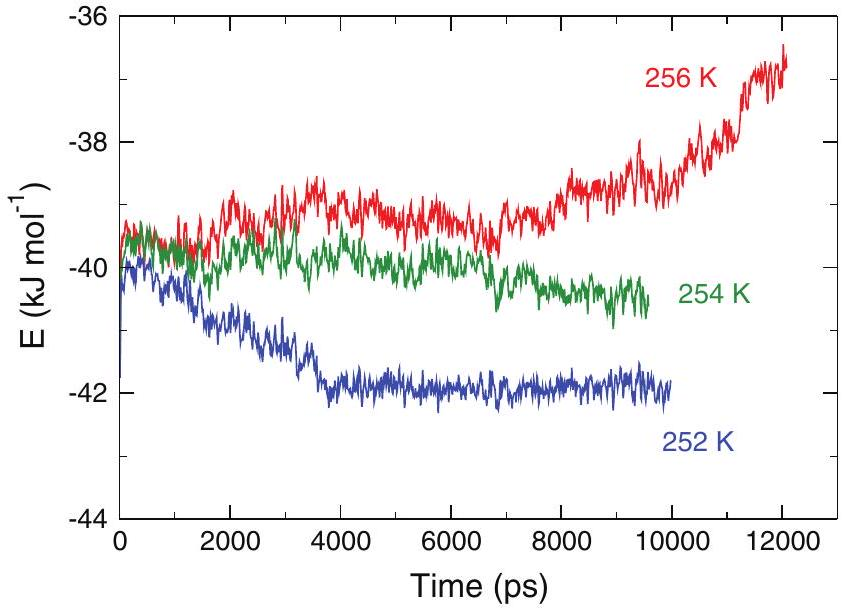
\includegraphics[alt={},max width=\textwidth]{a79b7aee-e943-46ce-b653-92f3182dbe04-6_609_846_176_1095}
\captionsetup{labelformat=empty}
\caption{FIG. 5. Evolution of the total energy of a system made of liquid water in contact with ice Ih. The results are averages over 20 ps simulation blocks for three $N p T$ simulation runs at 1 bar and $T=256 \mathrm{~K}, 254 \mathrm{~K}$, and 252 K , respectively.}
\end{center}
\end{figure}

\section*{G. Relative stability of ices}
It has been shown recently that the relative stability of the ice polymorphs is not correctly predicted be several rigid water models. ${ }^{18,45}$ In particular, the stable phase at ambient conditions of three site models such as TIP3P, SPC, or SPC/E is not the hexagonal ice Ih but the proton ordered ice II. The calculation of the complete phase diagram is outside the scope of this work but there is a simple alternative consisting in the calculation of the relative stabilities at $0 \mathrm{~K} .{ }^{53}$ Table V presents the densities and energies of ices Ih, II, III, and VI for the flexible models TIP4P/2005f and SPC/Fw as well as for their rigid counterparts TIP4P/2005 and SPC/E. Both TIP4P/2005 and TIP4P/2005f predict ice Ih as the more stable phase while ice II is more stable for SPC/E and SPC/Fw indicating that the flexibility has a small influence on the relative stability of ices. In this respect, it is perhaps worth to mention the slight increased stability of ice III which is marginally more stable than ice II at 0 K for TIP4P/2005f. This means that ice II would be absent from the phase diagram of this model. This is in accordance with a recent calculation for a flexible model (also based on TIP4P/2005) designed to be used

\begin{table}[h]
\begin{center}
\captionsetup{labelformat=empty}
\caption{TABLE V. Properties of several ice polymorphs at $T=0 \mathrm{~K}$ and $p=0$ bar for flexible water models and their rigid counterparts. The results marked in bold correspond to the more stable phase.}
\begin{tabular}{|l|l|l|l|l|}
\hline
Ice & TIP4P/2005 & TIP4P/2005f & SPC/E & SPC/Fw \\
\hline
\multicolumn{5}{|c|}{U (kcal/mol)} \\
\hline
Ih & -15.06 & -14.76 & -14.69 & -14.64 \\
\hline
II & -14.85 & -14.49 & -14.85 & -14.80 \\
\hline
III & -14.74 & -14.52 & -14.35 & -14.26 \\
\hline
VI & -14.51 & -14.20 $\rho\left(\mathrm{g} / \mathrm{cm}^{3}\right)$ & -13.95 & -13.85 \\
\hline
Ih & 0.954 & 0.961 & 0.981 & 0.996 \\
\hline
II & 1.230 & 1.232 & 1.279 & 1.295 \\
\hline
III & 1.184 & 1.189 & 1.181 & 1.214 \\
\hline
VI & 1.385 & 1.390 & 1.413 & 1.434 \\
\hline
\end{tabular}
\end{center}
\end{table}

\begin{table}[h]
\begin{center}
\captionsetup{labelformat=empty}
\caption{TABLE VI. Dielectric constant at different thermodynamics states.}
\begin{tabular}{|l|l|l|l|l|}
\hline
$T(\mathrm{~K})$ & $p$ (bar) & TIP4P/2005 & TIP4P/2005f & Expt. \\
\hline
298 & 1 & 57.2 & 55.3 & 78.4 \\
\hline
298 & 2000 & 62.2 & 63.1 & 84.9 \\
\hline
473 & 2000 & 31.8 & 33.0 & 41.3 \\
\hline
673 & 2000 & 16.6 & 16.7 & 19.4 \\
\hline
\end{tabular}
\end{center}
\end{table}

in simulations explicitly accounting for the quantum nuclear motion. ${ }^{54}$

The fact that SPC/Fw is unable to predict the relative stabilities of ices Ih and II is a serious drawback of the model and supports our decision to develop a flexible model based on TIP4P/2005. It may be argued that the properties of water in the solid state are not important because these models are intended to be used for the liquid state. But this is a simplification because it is now well documented that the relative stability of ice II with respect to the other proton disordered polymorphs (Ih, III, V, and VI) is related to the ratio between the magnitudes of the dipole and quadrupole moments of the model. ${ }^{20,21}$ Thus, the failure of SPC/Fw in accounting for the relative stability of ices Ih and II is not a simple inadequacy for the study of ices but it has deeper roots with consequences also for the liquid state.

\section*{H. Static dielectric constant}
The static dielectric constant is one of the few properties for which the TIP4P/2005 model does not provide a satisfactory result. The appropriate equation for its computation in a simulation using Ewald sums with conducting boundary conditions reads ${ }^{55}$


\begin{equation*}
\varepsilon_{r}=1+\frac{4 \pi}{3 k_{B} T V}\left(\left\langle M^{2}\right\rangle-\langle M\rangle^{2}\right) . \tag{9}
\end{equation*}


In order to compute the dielectric constant we have performed several simulation in the NVE ensemble lasting 15 ns . It seems interesting to check not only the values of the dielectric constant but also how the model is able to predict its change for different thermodynamic states. Table VI presents the dielectric constant for several points along the 298 K isotherm and the 1000 bar isobar. The results for the flexible model follow the same trends as the experimental values but the error is considerable. Besides the dielectric constants of the flexible model are quite similar to those of the rigid one; except for the point at ambient conditions there is a marginal improvement associated to the addition of flexibility.

\section*{I. Power spectrum}
There are several methods to calculate the infrared spectrum. We used a method based on the computation of the density of states or the power spectra. ${ }^{56}$ This involves the Fourier transform of the velocity autocorrelation function (VAC) for the relative velocities of a hydrogen atom with respect to the oxygen atom, ${ }^{56-58}$


\begin{equation*}
I(\omega) \propto \int_{0}^{\infty} d t \exp (-i \omega t)\langle v(0) v(t)\rangle \tag{10}
\end{equation*}


\begin{figure}[h]
\begin{center}
  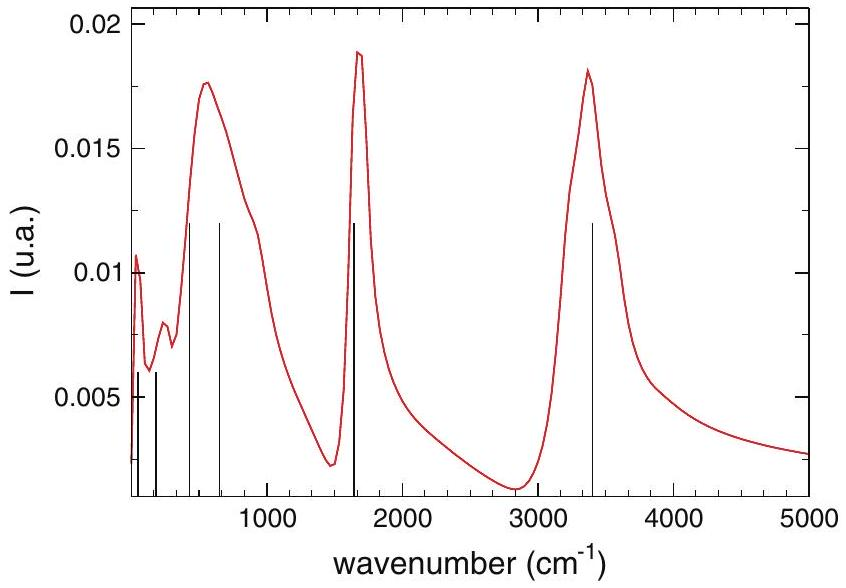
\includegraphics[alt={},max width=\textwidth]{a79b7aee-e943-46ce-b653-92f3182dbe04-7_588_846_171_1095}
\captionsetup{labelformat=empty}
\caption{FIG. 6. Spectrum of densities of state of water. Vertical lines signal the position of the peaks in the experimental spectra of liquid water.}
\end{center}
\end{figure}

where $\langle v(0) v(t)\rangle$ is the velocity autocorrelation function and $\omega$ is the frequency. This method allows one to obtain the values of the maximum of the bands at a much lower computational cost than the traditional method based on the dipole moment of the system. This is sufficient to verify the validity of the model but if one wants to improve the calculation of the infrared spectrum, quantum corrections ${ }^{33}$ or, better, advanced methods based on quantum calculations ${ }^{59-63}$ are required. To obtain this information of the system, we have used specific simulation conditions. The required simulation time is quite short, only 10 ps , because of the rapid decay of the VAC but a small time-step, 0.1 fs , is needed to define precisely the VAC at very short times. Besides this, a larger system (4000 molecules) is necessary to eliminate noise and to obtain accurate values for $I(\omega)$.

Figure 6 displays the profile of the spectrum of densities of states of water. We have also included in the plot the positions of the peaks of the experimental bands. As expected, the frequency at the maximum for the angle bending and the bond stretching are more or less coincident with the experimental values. The bands corresponding to the librational motion with symmetries A2, B2 are merged together in a single band whose maximum appears approximately at the middle point of the experimental peaks. ${ }^{65}$ The intramolecular stretch is somewhat shifted towards higher frequencies. It is to be noticed that the band at about $50 \mathrm{~cm}^{-1}$ appears clearly resolved in our model and that is maximum, and is coincident with the experimental value. The peaks of the bands of the power spectrum are collected in Table VII where we compare it with experimental measurements. ${ }^{37,64,65}$

\begin{table}[h]
\begin{center}
\captionsetup{labelformat=empty}
\caption{TABLE VII. Wavenumbers (in $\mathrm{cm}^{-1}$ ) at the peak of the bands of the power spectrum for the TIP4P/2005f model and liquid water. Experimental results have been taken from Refs. 37 and 64-66.}
\begin{tabular}{|l|l|l|}
\hline
 & TIP4P/2005f & Expt. \\
\hline
Cage vibrations ${ }^{9}$ & 50 & 50 \\
\hline
Intermolecular stretch & 230 & 183.4 \\
\hline
Librations A2, B2 & 570 & 430,650 \\
\hline
Bending ( $\mathrm{H}-\mathrm{O}-\mathrm{H}$ ) & 1670 & 1643.5 \\
\hline
Stretching ( $\mathrm{O}-\mathrm{H}$ ) & 3370 & 3404.0 \\
\hline
\end{tabular}
\end{center}
\end{table}

\section*{IV. CONCLUSIONS}
In this work we have developed a flexible water model, TIP4P/2005f, based on the rigid potential TIP4P/2005. A number of structural, thermodynamic and dynamic properties have been evaluated for the new model. Most of the results are in excellent agreement with experiment in line with as those of its rigid predecessor. Taking into account the excellent performance of TIP4P/2005 for other properties not evaluated in this work, this seems to ensure that TIP4P/2005f is a very accurate flexible model. The model slightly improves the melting point and there are also marginal improvements in other properties. On the negative side, although the results for the dielectric constant follow similar trends as the experimental ones, they are still considerably different from experiment. In summary, the flexible TIP4P/2005f seems to inherit the excellent performance of TIP4P/2005 but it does not improve it substantially. We must conclude that adding flexibility does not improve the performance for those properties for which the predictions of TIP4P/2005 are not quantitative.

The reasoning of the preceding paragraph seems to be in contradiction with several reports claiming that some predictions of flexible models are closer to experimental data than those of rigid potentials. ${ }^{12,15}$ It seems that the flexibility has more influence on the final results (at least for a few number of properties) when the model is based on SPC/E than for a model based on TIP4P/2005. The reasons of this different behavior are unclear to us but this might be simply because the TIP4P/2005 results are already very good so its improvement is not an easy task. It was not the objective of this work to compare the results of TIP4P/2005f to those of other flexible models. We have calculated the relative stability of ices just to confirm that our choice on using a TIP4P topology as the starting point of a flexible model was based on correct premises. We have shown that SPC/Fw predicts erroneously that ice Ih is less stable than ice II. Moreover, given the value of the expansivity reported by Wu et al., ${ }^{11}$ it is likely that the temperature of maximum density for SPC/Fw is far from the experimental value (following the behavior of SPC/E for which the maximum density is reached at $241 \mathrm{~K}, 36^{\circ}$ below the experimental value). TIP4P/2005f is free from these drawbacks and its performance is excellent even if the addition of flexibility does not improve substantially that of TIP4P/2005. It is then a good candidate in simulations where the use of a flexible water model is advisable.

\section*{ACKNOWLEDGMENTS}
This work has been funded by grants FIS2010/16159 of the MEC, P2009/ESP-1691 of CAM and UCM-Banco de Santander GR35/10-A-910570.

\footnotetext{${ }^{1}$ B. Guillot, J. Mol. Liq. 101, 219 (2002).\\
${ }^{2}$ C. Vega and J. L. F. Abascal, Phys. Chem. Chem. Phys. 13, 19663 (2011).\\
${ }^{3}$ D. E. Smith and A. D. J. Haymet, J. Chem. Phys. 96, 8450 (1992).\\
${ }^{4}$ I. G. Tironi, R. M. Brunne, and W. F. van Gunsteren, Chem. Phys. Lett. 250, 19 (1996).\\
${ }^{5}$ B. S. Gonzalez, E. G. Noya, C. Vega, and L. M. Sese, J. Phys. Chem. B 114, 2484 (2010).\\
${ }^{6}$ I. Kurisaki and T. Takahashi, Comput. Theor. Chem. 966, 26 (2011).
}
${ }^{7}$ S. Habershon, T. E. Markland, and D. E. Manolopoulos, J. Chem. Phys. 131, 024501 (2009).\\
${ }^{8}$ J. Marti, E. Guardia, and J. A. Padro, J. Chem. Phys. 101, 10883 (1994).\\
${ }^{9}$ J. Marti, J. A. Padro, and E. Guardia, J. Chem. Phys. 105, 639 (1996).\\
${ }^{10}$ U. W. Schmitt and G. A. Voth, J. Phys. Chem. B 102, 5547 (1998).\\
${ }^{11}$ Y. J. Wu, H. L. Tepper, and G. A. Voth, J. Chem. Phys. 124, 024503 (2006).\\
${ }^{12}$ G. Raabe and R. J. Sadus, J. Chem. Phys. 134, 234501 (2011).\\
${ }^{13}$ G. Raabe and R. J. Sadus, J. Chem. Phys. 126, 044701 (2007).\\
${ }^{14}$ J. Lopez-Lemus, G. A. Chapela, and J. Alejandre, J. Chem. Phys. 128, 174703 (2008).\\
${ }^{15}$ P. K. Yuet and D. Blankschtein, J. Phys. Chem. B 114, 13786 (2010).\\
${ }^{16}$ W. L. Jorgensen, J. Chandrasekhar, J. D. Madura, R. W. Impey, and M. L. Klein, J. Chem. Phys. 79, 926 (1983).\\
${ }^{17}$ H. J. C. Berendsen, J. R. Grigera, and T. P. Straatsma, J. Phys. Chem. 91, 6269 (1987).\\
${ }^{18}$ E. Sanz, C. Vega, J. L. F. Abascal, and L. G. MacDowell, Phys. Rev. Lett. 92, 255701 (2004).\\
${ }^{19}$ J. L. F. Abascal and C. Vega, Phys. Chem. Chem. Phys. 9, 2775 (2007).\\
${ }^{20}$ J. L. F. Abascal and C. Vega, Phys. Rev. Lett. 98, 237801 (2007).\\
${ }^{21}$ J. L. F. Abascal and C. Vega, J. Phys. Chem. C 111, 15811 (2007).\\
${ }^{22}$ J. L. F. Abascal and C. Vega, J. Chem. Phys. 123, 234505 (2005).\\
${ }^{23}$ H. L. Pi, J. L. Aragones, C. Vega, E. G. Noya, J. L. F. Abascal, M. A. Gonzalez, and C. McBride, Mol. Phys. 107, 365 (2009).\\
${ }^{24}$ C. Vega, J. L. F. Abascal, and I. Nezbeda, J. Chem. Phys. 125, 034503 (2006).\\
${ }^{25}$ L. Pusztai, O. Pizio, and S. Sokolowski, J. Chem. Phys. 129, 184103 (2008).\\
${ }^{26}$ F. Sedlmeier, D. Horinek, and R. R. Netz, J. Am. Chem. Soc. 133, 1391 (2011).\\
${ }^{27}$ M. A. Gonzalez and J. L. F. Abascal, J. Chem. Phys. 132, 096101 (2010).\\
${ }^{28}$ G. Guevara-Carrion, J. Vrabec, and H. Hasse, J. Chem. Phys. 134, 074508 (2011).\\
${ }^{29}$ J. L. F. Abascal and C. Vega, J. Chem. Phys. 134, 186101 (2011).\\
${ }^{30}$ R. B. Best and J. Mittal, J. Phys. Chem. B 114, 14916 (2010).\\
${ }^{31}$ O. Teleman, B. Jonsson, and S. Engstrom, Mol. Phys. 60, 193 (1987).\\
${ }^{32}$ J. L. Barrat and I. R. McDonald, Mol. Phys. 70, 535 (1990).\\
${ }^{33}$ B. Guillot, J. Chem. Phys. 95, 1543 (1991).\\
${ }^{34}$ A. Wallqvist and O. Teleman, Mol. Phys. 74, 515 (1991).\\
${ }^{35}$ H. L. Lemberg and F. H. Stillinger, J. Chem. Phys. 62, 1677 (1975).\\
${ }^{36}$ K. Toukan and A. Rahman, Phys. Rev. B 31, 2643 (1985).\\
${ }^{37}$ J.-J. Max and C. Chapados, J. Chem. Phys. 131, 184505 (2009).\\
${ }^{38}$ J. E. Bertie and Z. D. Lan, Appl. Spectrosc. 50, 1047 (1996).\\
${ }^{39}$ C. P. Lawrence and J. L. Skinner, Chem. Phys. Lett. 372, 842 (2003).\\
${ }^{40}$ B. Hess, C. Kutzner, D. van der Spoel, and E. Lindahl, J. Chem. Theory Comput. 4, 435 (2008).\\
${ }^{41}$ D. van der Spoel, E. Lindahl, B. Hess, G. Groenhof, A. E. Mark, and H. J. C. Berendsen, J. Comput. Chem. 26, 1701 (2005).\\
${ }^{42}$ G. Bussi, D. Donadio, and M. Parrinello, J. Chem. Phys. 126, 014101 (2007).\\
${ }^{43}$ M. Parrinello and A. Rahman, J. Appl. Phys. 52, 7182 (1981).\\
${ }^{44}$ U. Essmann, L. Perera, M. L. Berkowitz, T. A. Darden, H. Lee, and L. G. Pedersen, J. Chem. Phys. 103, 8577 (1995).\\
${ }^{45}$ C. Vega, J. L. F. Abascal, M. M. Conde, and J. L. Aragones, Faraday Discuss. 141, 251 (2009).\\
${ }^{46}$ A. K. Soper, Chem. Phys. 258, 121 (2000).\\
${ }^{47}$ R. Mills, J. Phys. Chem. 77, 685 (1973).\\
${ }^{48}$ K. Krynicki, C. D. Green, and D. W. Sawyer, Faraday Discuss. Chem. Soc. 66, 199 (1978).\\
${ }^{49}$ K. T. Gillen, D. C. Douglass, and M. J. R. Hoch, J. Chem. Phys. 57, 5117 (1972).\\
${ }^{50}$ R. García Fernández, J. L. F. Abascal, and C. Vega, J. Chem. Phys. 124, 144506 (2006).\\
${ }^{51}$ A. Ladd and L. Woodcock, Chem. Phys. Lett. 51, 155 (1977).\\
${ }^{52}$ J. R. Morris and X. Song, J. Chem. Phys. 116, 9352 (2002).\\
${ }^{53}$ J. L. Aragones, E. G. Noya, J. L. F. Abascal, and C. Vega, J. Chem. Phys. 127, 154518 (2007).\\
${ }^{54}$ S. Habershon and D. E. Manolopoulos, Phys. Chem. Chem. Phys. 13, 19714 (2011).\\
${ }^{55}$ M. Neumann, Mol. Phys. 50, 841 (1983).\\
${ }^{56}$ M. P. Allen and D. J. Tildesley, Computer Simulation of Liquids (Oxford University Press, Oxford, 1987).\\
${ }^{57}$ D. A. McQuarrie, Statistical Mechanics (University Science Books, Sausalito, 2000).\\
${ }^{58}$ S. Amira, D. Spangberg, and K. Hermansson, Chem. Phys. 303, 327 (2004).\\
${ }^{59}$ G. S. Fanourgakis and S. S. Xantheas, J. Chem. Phys. 128, 074506 (2008).\\
${ }^{60}$ J. L. Skinner, B. M. Auer, and Y.-S. Lin, Adv. Chem. Phys. 142, 59 (2009).\\
${ }^{61}$ B. M. Auer and J. L. Skinner, Chem. Phys. Lett. 470, 13 (2009).\\
${ }^{62}$ M. Yang and J. L. Skinner, Phys. Chem. Chem. Phys. 12, 982 (2010).\\
${ }^{63}$ C. Zhang, D. Donadio, F. Gygi, and G. Galli, J. Chem. Theory Comput. 7, 1443 (2011).\\
${ }^{64}$ G. E. Walrafen, J. Chem. Phys. 40, 3249 (1964).\\
${ }^{65}$ D. M. Carey and G. M. Korenowski, J. Chem. Phys. 108, 2669 (1998).\\
${ }^{66}$ M. Chaplin, see \href{http://www.lsbu.ac.uk/water}{http://www.lsbu.ac.uk/water}. A site about the structure, function, behavior and properties of water.


\end{document}